\chapter{Discussion}
\label{chap:discussion}
This chapter highlights the implemented methods' capability to handle a variety of testcases, as well as current limitations and challenges of the implemented methods, focusing on their impact on error detection, visualization, and overall system efficiency.

\section{Testcases}
As seen in \autoref{chap:evaluation}, all 20 unique testcases are correctly identified and indicated to the user and, as seen in \autoref{tab:functional_test_cases_no_errors}, no errors are reported if none are simulated.\\
In the \textit{free floating star} test case, error detection is straightforward, as the star is detected in the tokenization step and highlighted. In the \textit{input instead of output} and \textit{free floating input / \acrshort{io}} testcases, all vertices are known, but they are not correctly positioned, resulting in an error indication during the syntax step of the pipeline. Similar error indications are generated in the \textit{text too far} and \textit{text too near} test cases, because they too are correctly identified during tokenization but have a slightly shifted position, resulting in syntax errors.

\begin{wrapfigure}{r}{0.4\textwidth}
    \centering
    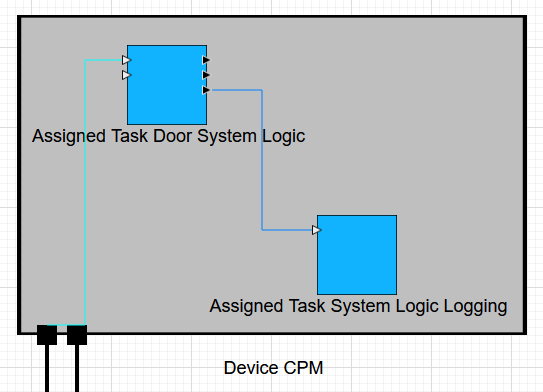
\includegraphics[width=0.4\textwidth]{pictures/allocations_thin_edges.png}
    \caption{Example of the thin edges in the allocations editor, which are hard to detect using the currend edge detection method.}
    \label{fig:allocations_thin_edges}
\end{wrapfigure}
In \textit{device wrong color}, \textit{task wrong color} and \textit{signal wrong color}, the color of one of the vertices or edges is changed such, that it is no longer being detected in the tokenization step. This results in untokenized pixels, as well as a number of additional errors, because for example, the associated \acrshort{io} ports of the changed device are now seemingly floating in space, resulting in wrong syntax. The same problem arises in the simulated testcases \textit{task / device too small}.

Further problems arise when instantiating and comparing the new model without the changed device. These additional errors are reported, making it harder for the user to identify the original problem cause.\\
Furthermore, as illustrated in \autoref{tab:functional_test_cases_no_errors}, a changed color is only reported as an error, if the intensity of the original and altered color is significantly different. This is because \acrshort{opencv}'s \textit{matchtemplate} function compares the pixels intensities, effectively ignoring colors. This could be improved by running the template matching algorithm seperately for each color channel and then comparing the results or by incorporating a different method more suitable for differentiating color hues.

\section{Limitations of current Methods}
The current implementation is, in large parts, model driven, meaning it can recognize the current model and query it for information, such as a list of the used token types and the location of their respective \textit{.svg} files.\\
However, a current limitation is the amount of information that can be queried and utilized. For instance, the current implementation does not query the current model layer, making it difficult to differentiate between \textit{function}-, \textit{hardware}-, and \textit{allocation} layers. This can lead to less efficient tokenization. For example, during text recognition, the image is searched for rotated text, regardless of whether the current model contains any.\\
Another limitation lies in the template matching method. As stated in \autoref{chap:new_concepts}, the current implementation applies each template to the image, which works well if the used templates are stored within the model, enabling the system to query them and dynamically choose the correct templates for each model layer. However, for edge and intersection detection, no such convenient template files are stored. Instead, the templates are generated with a fixed size, making it harder to adapt the system to changes in edge width, color, or intersection visualizations.\\
Another limitation stems from the both the visualization and the edge detection pipeline's difficulty in identifying the edges connecting subtasks within the allocations editor (see \autoref{fig:allocations_thin_edges}). This is because these edges are too thin and lack sufficient contrast for accurate detection. Implementing a more robust algorithm or designing a visualization that is easier to detect for computer vision algorithms could enhance the detection process, potentially allowing it to be integrated into the edge detection pipeline.\\
Another limiting factor is the lack of error handling mechanisms. If an error occurs during the verification, it can disrupt or stop the entire workflow. Furthermore, a single error can result in many error indications, as discussed in \autoref{chap:discussion}, hampering the user's ability to quickly find the root cause of the error indications.

All of these limitations could be addressed by enhancing the current implementation with additional features, such as querying the model for more information, dynamically generating templates, or implementing more robust error handling mechanisms.\\


\chapter{Outlook}
\label{chap:outlook}
This chapter explores potential improvements and future directions for the methods and tools introduced in this thesis, with a focus on insights gained from the analysis of test cases. While the proposed edge, vertex, and text detection algorithms perform reliably in most scenarios, certain limitations became evident when applied to complex or ambiguous test cases.

\section{Edge Detection Further Improvements}
\label{sec:edge_detection_further_improvements}
The method introduced in this thesis successfully detects and processes nearly all edges within \acrshort{xgee}. In contrast to the previous algorithm, it can identify edges in any orientation, regardless of their start or endpoint or order of their line segments. Furthermore, it is capable of processing and interpreting intersections and signal containers, making it well-suited for handling large, complex models. The method performs reliably across all three editor models, provided the models are formatted correctly (the zoom level has to be set to 100\% across the entire operating system for the edge detection to work reliably). In cases where multiple edges overlap or many intersections are within a few pixels of each other, an error is reported, as the method, as well as human operators, can not reliably interpret the image. This enforces an unambiguous model layout, which is achieved by either an automatic arrangement algorithm or the user.

The current intersection detection relies on a very specific visualization, where intersecting lines simply cross. This poses a limitation, as the method cannot adapt if the intersection visualization changes, for instance, to better display the intersection of multiple edges. A potential solution to this problem could involve extracting the intersection graphic from the screenshot by predicting the intersection's position based on the detected edges. This approach would enable the method to adapt to different intersection visualizations, as long as the edges remain detectable.

A notable problem arises when vertices with surrounding black edges, such as devices or functions, are scaled sufficiently, making their edges resemble signal-carrying edges (see \autoref  {tab:functional_test_cases_no_errors}). This complicates their differentiation. In this case, a possible solution would be to let the vertex detection run first and exclude the found areas when applying the edge detection. Alternatively, the presence of colored pixels around the edges could be checked more thoroughly, as the background around edges is typically white, unlike the areas inside device or function vertices. This way, any obstructions caused by the vertices can be avoided.\\
Another issue may arise if the edges are configured by the user in an unexpected way. For instance, an intersection hidden behind vertices or signal containers cannot be properly interpreted by the current method, which could lead to unexpected results. Future improvements to the \acrshort{xgee} editor, such as a more advanced automatic arrangement algorithm, could reduce or eliminate the risk of ambiguous user input that would result in such cases. Another potential solution would be to search for edges along the sides of detected devices and functions and attempt to connect them. However, this approach might fail if multiple edges run behind a single device or function, which would also make the visualization difficult for a human user to interpret.

Another issue arises from edges connecting subtasks within the allocations editor. They often overlap with text, are too thin, and have too little contrast to be detected accurately. In a future version of \acrshort{xgee}'s visualization, enhancing the readability of subtask edges would enable a computer vision algorithm to detect them reliably, enabeling useful user feedback and thus improving the verification tool.

\section{Vertex Detection Further Improvements}
\label{sec:vertex_detection_further_improvements}
The proposed method can reliably detect almost all vertices across all of \acrshort{xgee}'s model layers, regardless of their dimensions or placement. It can effectively distinguish between subvertices and main vertices by querying the model and applying the appropriate template matching algorithm based on the properties of each template. Additionally, the current editor model is queried to identify the set of utilized vertices, which are subsequently detected. This adaptability enhances both the efficiency and reliability of the method, enabling it to handle changes in the model.\\
As described in \autoref{chap:new_concepts}, the current method identifies each token type within the allocation layer by following a structured detection sequence. First, subtasks are identified and subsequently erased from the screenshot to prevent interference with the detection of underlying vertices.\\
Currently, this approach is only used to enable the detection of devices in the allocations layer. In the future, extending this approach across the entire tokenization pipeline could significantly enhance vertex detection, ensuring that no vertices are obscured, no vertex is detected multiple times, and similar vertices, edges, or text are not mistakenly identified as one another.\\
To implement this improvement, the following steps could be taken:

\begin{itemize}
    \item Process all vertices, edges and text in hierarchical top-down order, starting with subvertices and ending with the main vertices, followed by text and edges.
    \item Query the parent vertex's main color and use it to erase all found vertices.
    \item Dynamically update the input image after each iteration and pass it to the next step in the tokenization pipeline.
    \item Correctly handle cases where subvertices, such as \acrshort{io} ports, only partially overlap with their parent vertices.
\end{itemize}

This approach would systematically simplify the screenshot with each step of the tokenization pipeline, effectively only leaving the untokenized pixels on a white background in the end. After the vertex detection step, the remaining pixels would be passed to the text detection algorithm, which would then identify any remaining text. Finally, the edge detection algorithm would process the remaining pixels, detecting any edges without the possibility of interference from other vertices. This approach would, however, require a way to deal with overlapping text labels, as they would most likely be partially removed in previous steps, making it impossible to properly recognize them.\\

Another possible improvement could be made by enabeling the current method to detect subvertices of subtasks (very small inputs and outputs, as seen in \autoref{fig:allocations_thin_edges}), which are currently excluded from detection due to their small size. These \textit{subsubvertices} are challenging to differentiate from noise, character fragments, or edge segments using \acrshort{opencv}'s built in methods. Employing image preprocessing techniques or refining or exchanging the template matching method could improve the detection of these smaller elements and thus enable a more precise visualization verification.

\section{Text Detection Future Improvements}
\label{sec:text_detection_future_improvements}
Currently, the text recognition system can detect almost any text present within \acrshort{xgee}. Regardless of the current editor, the screenshot is rotated and analyzed to identify any rotated text, which contributes to text detection being the most time consuming component of the visualization verification process.

Optimizing the performance of the text detection algorithm would significantly reduce the overall processing time. This could be achieved by identifying the specific editor type to allow the system to selectively search for rotated characters only when they are expected to be present in the image. Additionally, running the visualization verification on a \acrshort{gpu}, parallelizing the text detection to run simultaneous to the edge- and vertex detection or using a more traditional text detection algorithm which does not require as much computational power as Easy\acrshort{ocr} would enable the system to process larger models more quickly and efficiently, addressing the current bottleneck in the pipeline.\\
Currently, the average runtime of the verification pipeline on an Intel Core Ultra 9 185H \acrshort{cpu} is 54 seconds, with 76\% of runtime spent on character recognition.\\
A new \acrshort{ocr} model would also potentially allow for a more precise way to filter out falsely read characters instead of removing every recognized word shorter than three letters.

Another potential improvement could be made regarding the text recognition's accuracy. Currently, the method is limited by the quality of the input image and the Easy\acrshort{ocr} library. This is because most \acrshort{ocr} engines are trained on books, where text is orderly structured and has a predictable orientation. In contrast, the text in \acrshort{xgee} models is often rotated, distorted, or partially occluded, making it difficult for the \acrshort{ocr} engine to recognize. Additionally, individual numbers are hard for Easy\acrshort{ocr} to detect reliably.\\
Training a custom \acrshort{ocr} model on a dataset of \acrshort{xgee} text images could improve the recognition accuracy, as the model would be specifically tailored to the unique characteristics of \acrshort{xgee} text. In future implementations, this could be achieved by automatically generating the training data alongside the correct text by directly querying the model.\\
A simpler way to solve the problem of wrongly detected characters could be improved error handeling, to indicate these types of errors to the user in a simple and clean way. This would enable the user to quickly identify and correct any false errors, reducing the time spent on verification.

\section{Expanding to other Domains or Applications}
\label{sec:expanding_to_other_domains}
As described in \autoref{chap:evaluation}, the current implementation is optimized to work model driven in the functions- and hardware layer. Further working on the implementation into the allocations layer would be a logical next step, fully enabeling the verification tool to work with all three of \acrshort{xgee}'s editors, dynamically changing with the model. However, because of the higher complexity of the allocations layer, this would require restructuring the current implementation to consider the order of detection and the hierarchical structure of the model in all steps of the verification pipeline.

One of the goals of this thesis was to generalize the used tokenization algorithms to work in all three of \acrshort{xgee}'s editors. Expanding upon this idea, a future verification pipeline could be able to understand a wide range of different editors, potentially enabeling the verification of editors completely seperated from the verification program. This could be achieved by implementing a more general tokenization pipeline, which could be configured to work with any editor, given the correct templates and cofiguration files.\\
Enabeling the verification to work with editor models like Simulink and other widely used modeling tools would make the verification tool more versatile and useful to a wide audience, potentially resulting in an increase in demand for automatic visualization verification tools.